\documentclass{article}
\usepackage[utf8]{inputenc}
\usepackage{amsmath, amssymb}
\usepackage[margin=1.0in]{geometry}
\usepackage{graphicx}
\usepackage{mathrsfs}
\usepackage{hyperref}
\usepackage{float}

\title{Note of Fast Runner}
\author{Ken}
\date{June, 2018}

\usepackage{natbib}
\usepackage{graphicx}
\graphicspath{ {./images/} }
\usepackage{amsthm}


\newtheorem{prop}{Proposition}

\begin{document}

\maketitle
\section{System dynamics}
\begin{figure}[h]
\centering

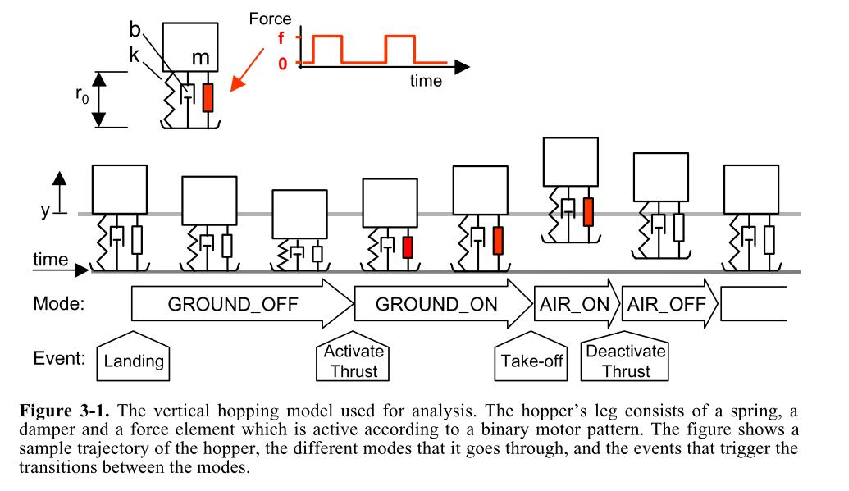
\includegraphics{test.pdf} 
\caption{The schematic of a 1 DOF hopper \cite{Cham2002}}
\label{fig.1DOF-Hopper}
\end{figure}
\subsection{Sequence}
\{AIR\_OFF, GROUND\_OFF, GROUND\_ON, AIR\_ON\}


\subsection{Equation of motion}
Using the model as shown in Fig. \ref{fig.1DOF-Hopper}, during the stand phase (i.e. $y\leq 0$), the equation of motion can be expressed as:
\begin{align*}
m \ddot y = -b\dot y +-ky -mg + f
\end{align*}
\noindent where $m$ is the mass, $b$ is the damping, $k$ is the stiffness, $f$ is the control input.
Normalized by weight, the equation becomes
\begin{align*}
 \ddot y = -b/m\dot y +-k/my -g + f/m
\end{align*}

\noindent Expressed in state space form:

\begin{align}
\begin{bmatrix}
\dot y  \\
\ddot y 
\end{bmatrix} = \begin{bmatrix}
0 & 1 \\
-k/m & -b/m
\end{bmatrix}\begin{bmatrix}
 y  \\
\dot y 
\end{bmatrix} + 
\begin{bmatrix}
0  \\
-g+f/m 
\end{bmatrix}
\end{align}
or equivalently
\begin{align}
\label{eq:groundEOM}
\dot X = \begin{bmatrix}
0 & 1 \\
-\omega^2 & -2\xi\omega
\end{bmatrix}X + 
\begin{bmatrix}
0  \\
-g+f_n(t)
\end{bmatrix} &= AX+B
\end{align}
where $X \triangleq [y,\dot y]^T$.
When the hopper is in the air (i.e. $y> 0$, flight phase), 
\begin{align}
\label{eq:airEOM}
\dot X = \begin{bmatrix}
0 & 1 \\
0 & 0
\end{bmatrix}X + 
\begin{bmatrix}
0  \\
-g 
\end{bmatrix}
\end{align}
\noindent Define the force  of an open-loop motor pattern
\begin{align}
 f_n(t)=\begin{cases}
    f/m, & \text{if $t_{off}<t<t_{off}+t_{on}$}.\\
    0, & \text{otherwise}.
  \end{cases}
\end{align}

\noindent\textbf{Solutions}

For \eqref{eq:airEOM}:
\begin{align}
\label{eq:airEOMsol}
X(t) = \begin{bmatrix}
1 & t \\
0 & 0
\end{bmatrix}X_0 + 
\begin{bmatrix}
t^2/2  \\
 t
\end{bmatrix}(-g)
\end{align}

For \eqref{eq:groundEOM} when actuator is on:
\begin{align}
\label{eq:groundEOMsol}
X(t) = e^{At}(X_0-X_{eq_{on}}) + X_{eq_{on}}
\end{align}

For \eqref{eq:groundEOM} when actuator is off:
\begin{align}
\label{eq:groundEOMsol2}
X(t) = e^{At}(X_0-X_{eq_{off}}) + X_{eq_{off}}
\end{align}

where $X_{eq_{on}}$ and $X_{eq_{off}}$ are the equilibrium states:
\begin{align}
\label{eq:eqStates}
X_{eq_{on}} &= [\frac{f_n-g}{\omega^2}, 0]^T\\
X_{eq_{off}}&= [\frac{-g}{\omega^2}, 0]^T
\end{align}

\subsection{Stability Analysis}
\subsubsection{Eigen values}
For \eqref{eq:airEOM}, eigen values are $\pm 1$, in inherently unstable. (Why this does not matter? Because the contact)

\noindent For \eqref{eq:groundEOM}, eigen values are
$-\xi\omega \pm \omega\sqrt{(\xi^2-1)} = -\omega(\xi \pm \sqrt{\xi^2 -1}) = -\omega(\xi \pm i\sqrt{1-\xi^2 })$ As long as \omega  and \xi are larger than zero, the system is stable.

\subsubsection{Poincare Method}
\begin{figure}[H]
\centering

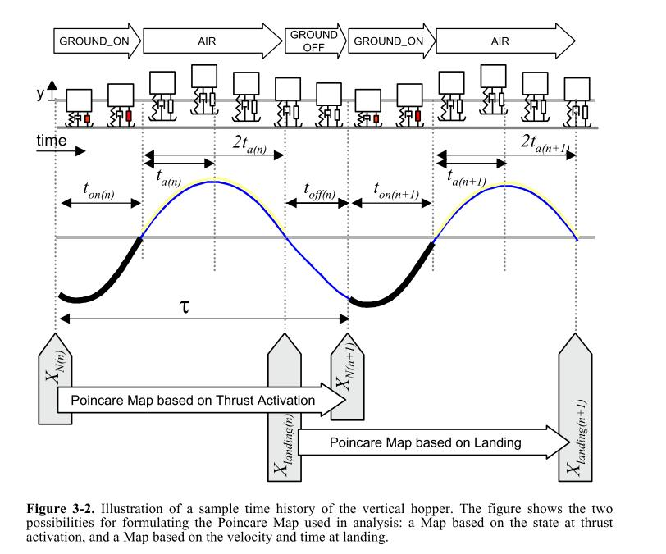
\includegraphics{modes.pdf} 
\caption{The modes of the hopper \cite{Cham2002}}
\label{fig.modes}
\end{figure}

Assumptions:
\begin{itemize}
\item the period is T
\item two modes need to be checked
\item $X(0) = X_{N_n}$ where $n$ indicates the $n^{th}$ trajectory
\end{itemize}

\noindent Using Equations \ref{eq:groundEOMsol}, we can derive
\begin{align*}
X(t_{on_n} )= e^{At_{on_n}}(X_{N_n} - X_{eq_{on}})+ X_{eq_{on}}
\end{align*}
\noindent Use the fact that 
\begin{align*}
X(t_{on_n}+2t_{a_n}) = -X(t_{on_n} ) 
\end{align*}

\noindent Then we can calculate the $X_{N_{n+1}}$ as follows:
\begin{align}
\nonumber X_{N_{n+1}} &= e^{A(T-2t_{a_n}-t_{on_n})}(-X(t_{on_n} ) - X_{eq_{off}}) + X_{eq_{off}}\\\
\nonumber X_{N_{n+1}} &= e^{A(T-2t_{a_n}-t_{on_n})}(-e^{At_{on_n}}(X_{N_n} - X_{eq_{on}})- X_{eq_{on}} ) - X_{eq_{off}}) + X_{eq_{off}}\\
&= X_{eq_{off}}-e^{A(T-2t_{a_n})}(X_{N_n}-X_{e_{on}}) -e^{A(T-2t_{a_n}-t_{on_n})}( X_{eq_{on}}+ X_{eq_{off}})
\end{align}

About the second switch surface $X_{landing_n}$,
\begin{align}
X_{landing_n} = -X(t_{on_n} ) =- e^{At_{on_n}}(X_{N_n} - X_{eq_{on}})- X_{eq_{on}}
\end{align}
\section{Code implementation}





\subsection{Modeling and Parameters}
Main idea: a virtual wheel (as the massless leg) with radius $r_{wheel}$ penetrate the ground for a distance $r_{pen}$ where a external force point $pe$ is attached on it. A body (with mass $m$ and inertia $Iyy$) is attached to the center of wheel. 
Using PD control to interpret contact force when $p_e$ is under the ground.

\subsubsection*{06/07 First prototype (Not used now)}
\begin{itemize}
\item Joint numbers: 2
\item Joint types: Floating planer joint for virtual wheel and pin joint for the body link.
\item Contact point type: External force point
\item Virtual wheel rotation: set proper initial condition for virtual wheel (also need a large inertia to make it nearly constant).
\end{itemize}

Contact force: Assuming the ground height is $0$,
\begin{align}
F_z &= kp(0-pe_z) + kd(0 - ve_z)\\
\phi &= atan2(pe_x,r_{wheel}-pe_z)\\
F_x &= F_ztan(\phi)
\end{align}
where $ve$ is the velocity vector of the contact point $pe$, $kp$ and $kd$ are the PD control parameters. $F_x$ is calculated so that the vector of ground reaction force $[F_x,F_y,F_z]^T$ will point towards the virtual pivot (the center of the virtual wheel).\\

Assessments:
\begin{itemize}
\item Need to set a non-zero inertia of massless virtual wheel (for numerical stability), otherwise the simulation will diverge.
\item The inertia of virtual wheel need to be a large one for constant rotational speed.
\item Suggestions: remove the massless link, attach the external force point to the body and change its position in the controller every time step.
\end{itemize}

\subsubsection*{06/08 Round Runner}
\begin{itemize}
\item Joint numbers: 1
\item Joint types: Floating planer joint for the body link.
\item Contact point type: External force point
\item Virtual wheel rotation: Assigning the external force point location with respect to the joint in an open loop manner.
\item 
Contact force: Assuming the ground height is $0$,
\begin{align}
F_z &= kp(0-pe_z) + kd(0 - ve_z)\\
\phi &= atan2(pe_x,r_{wheel}-pe_z)\\
F_x &= F_ztan(\phi)
\end{align}
where $ve$ is the velocity vector of the contact point $pe$, $kp$ and $kd$ are the PD control parameters. $F_x$ is calculated so that the vector of ground reaction force $[F_x,F_y,F_z]^T$ will point towards the virtual pivot (the center of the virtual wheel).\\
\end{itemize}



Assessments:
\begin{itemize}
\item The ground reaction force looks better, while the energy is not balanced (after a while it will move towards the negative $x$ direction)
\item The inertia of virtual wheel need to be a large one for constant rotational speed.
\item Suggestions: Use the ground contact point (instead of external force point) to see how it goes.

\end{itemize}

\subsubsection*{06/11 Round Runner(with Ground Contact Point)}
\begin{itemize}
\item Joint numbers: 1
\item Joint types: Floating planer joint for the body link.
\item Contact point type: Ground contact point, linear contact model\footnote[1]{Disable the hardening stiffness in z direction by setting groundStiffeningLength to Double.NEGATIVE\_INFINITY}
\item Virtual wheel rotation: Assigning the external force point location with respect to the joint in an open loop manner.
\item \textbf{Contact point number} Parameterized, currently set to 3-6 points.
\item
Contact force: using built-in functionalities, only assigning the $kp$, $kd$ (PD parameters in the z direction), $kp_x$, and $kd_x$ (PD parameters in the x/y directions).
\end{itemize}



Assessments:
\begin{itemize}
\item Was able to generate a stable walking. Contact point has sliding.
\item Due to setting up stiffness and damping for $x$ and $z$ separately, the force is not always point towards the virtual pivot.

\end{itemize}

\section{Info mightbe useful}

\subsection{Going through references}
\begin{enumerate}
\item Compare different terrestiral locomotions: Some parameters of the walk are not speed- dependent. The swing duration is a constant time parameter \cite{Abourachid2001}.
\item Trunk plays an important role during walking (birds) \cite{Abourachid2011}.
\item The use of these drives (Resonance drives, with adaptive control) allows increasing machine's quickness several times and decreasing energy expenses simultaneously 10-50 times \cite{Akinfiev1999}.
\item Light weight leg (ostrich vs. moa) can run faster\cite{Alexander1985}. Also a famous allometric equation:
\begin{align}
Y = M^{3/4}
\end{align}
where $M$ is the body mass, Y is the metabolic rate.
\item Human's walking may not be really self-optimized: the preferred speed maybe different from the energetically optimal speed\cite{Arnall2012}.
\item It is concluded that the most important adjustment to the body’s spring system to accommodate higher stride frequencies is that leg spring becomes stiffer \cite{Farley1996}.
\item magic equations for imd force (ostrich) \cite{Jindrich2007}
\item gait frequency was reported to be highly correlated with the resonant frequency of the mass-spring model \cite{Lee2013}
\item WABIAN, why you are here? \cite{Lim2008}
\end{enumerate}
\subsection{Categories}

\begin{enumerate}
\item Nonlinear oscillators/components \cite{Akinfiev1999,Anand1966,Babitsky1996,Buchli2006,Chatterjee2012, Karssen2011, Plooij2011};
\item zoology, biomechanics of animals:
\cite{Abourachid2001,Abourachid2011,Alexander1979,Alexander1985,Daley2007}
\item Bio-inspired robots: \cite{Ananthanarayanan2012,Lock2014}
\item Reference I should read: \cite{Cham2002,Daley2006,Kagawa2010,Karssen2011}
\item Article not found (or not free)\cite{Alexander1979}.
\item Robots in 3D: \cite{Coleman1997}
\item Stability analysis (Monocycle, linearized system) \cite{Coleman2010} (Limit cycle) \cite{Cham2002, Kagawa2010} dimensionless \cite{Riese2012}
\item Biology/Anatomical structure \cite{El-Mahdy2010,Gangl2004}
\item Light weight fast robot \cite{Ethington2013,Iida2012}
\item take a look again \cite{Gatesy1991}
\item mechanism design of robot \cite{Grimmer2011}
\item quadruped reference \cite{Hackert2001} MIT Cheetah\cite{Park2012}
\item human energy cost, resonance usage \cite{Holt1991,Arnall2012, Park2013, Racic2009}
\item walking parameterization \cite{Lee2008,Gatesy1991,Weems2006}
\item human-animal differences \cite{Daley2006}
\item open-loop robot \cite{Mombaur2005}, passive robot \cite{Owaki2011, Owaki2010, Owaki2009}
\end{enumerate}
%where x is a vector with n states (i.e. $x\in R^n$) called state variables, u is the control input, y the is control output, and A is a n by n matrix. Depends on the dimension of input and output, the system can be classified as single-input single-output (SISO) system or multi-input multi-output (MIMO) system.\\\\
%Other notes:
% \begin{itemize}
% \item For most of the systems that follow causality, the output has no instantaneous input (i.e. $D=[0]$).
% \item Time-invariant system (don't need to be linear) is also called \emph{autonomous system}. On the other hand, time-varying system is  called \emph{non-autonomous system}.
%\item When B=[0], the system is also called a \emph {unforced system}, as show in Eq \eqref{eqn:unforce}:
%\begin{align}
%\label{eqn:unforce}
%\dot {x}={A}x,
%\end{align}
%\end{itemize} 
%%
%\section{Solution for LTI system}
%\subsection{Laplace transform of a LTI system}
%Assume the initial condition of the state variable $x$ is $x_0$. By applying Laplace transform on both sides of Eq \eqref{eqn:unforce}:
%\[
%sX(s)-x_0=AX(s)\]
%\[\rightarrow(SI-A)X(s)=x_0\]
%\begin{align}
%\label{eqn:LA}
%\rightarrow X(s)=(SI-A)^{-1}x_0,
%\end{align}
%where $I$ is identity matrix. We can derive the Laplace transform  of $x$ : $X(s)$ as shown in Eq\eqref{eqn:LA}. By applying inverse Laplace transform on both sides of Eq\eqref{eqn:LA}, then the solution of LTI system can be derived as follows:
%\[
%\mathscr{L}^{-1}(X(s))=\mathscr{L}^{-1}((SI-A)^{-1}x_0)\]
%\begin{align}
%\label{eqn:sol}
%\rightarrow x(t)=\mathscr{L}^{-1}(\underbrace{(SI-A)^{-1}}_\text{resolvent matrix})x_0=e^{At}x_0
%\end{align}
%
%\subsection{Matrix exponential}
%For a arbitrary constant $a\in R$, $\mathscr{L}^{-1}(s-a)=e^{at}$. Similarly, if $A$ is a square matrix, $\mathscr{L}^{-1}(sI-A)=e^{At}$. The next coming question will be how to evaluate the \emph {matrix exponential} $e^{At}$? One way to go is using Taylor series expansion of the exponential function, which is shown as follows:\\\\
%For $a\in R$ is a constant,
%\[e^{at}=1+at+\frac{1}{2!}a^2t^2+\frac{1}{3!}a^3t^3+\ldots=
%\sum\limits_{k=1}^\infty \frac{1}{k!}a^kt^k\]
%For $A$ is a n by n matrix,
%\[e^{At}=I+At+\frac{1}{2!}A^2t^2+\frac{1}{3!}A^3t^3+\ldots=
%\sum\limits_{k=1}^\infty \frac{1}{k!}A^kt^k\]
%The Taylor series expansion of matrix exponential can also be used for verifying the solution of x:
%\[\dot x=\frac{dx}{dt}=\frac{d}{dt}e^{At}x_0\]
%\[\frac{d}{dt}e^{At}x_0=\frac{d}{dt}(I+At+\frac{1}{2!}A^2t^2+\frac{1}{3!}A^3t^3+\ldots)x_0\]
%\[\frac{d}{dt}e^{At}x_0=(A+A^2t+\frac{1}{2!}A^3t^2+\ldots)x_0\]
%\[\frac{d}{dt}e^{At}x_0=A(I+At+\frac{1}{2!}A^2t^2+\frac{1}{3!}A^3t^3+\ldots)x_0=Ax\]
%Matrix exponential $\Phi(0,t)=e^{At}$ is also called the \emph{state-transition matrix}\\
%(Please refer to: \url{https://en.wikipedia.org/wiki/State-transition_matrix} )
%
%\subsection{Solution of LTI system with control input}
%Considering the following derivative equation:
%\[\frac{d}{dt}(e^{-At}x(t))=-Ae^{-At}x+e^{-At}\dot x\]
%\[=e^{-At}(\dot x-Ax)\]
%\[=e^{-At}(Bu)\]
%Integrate the left hand side from $0$ to $t$:
%\[\int_{0}^{t} \frac{d}{dt}e^{-At}x(t)=[e^{-A\tau}x]_0^t=e^{-At}x(t)-x_0=\int_0^te^{-A\tau}Bu(\tau)d\tau\]
%\[\rightarrow e^{-At}x(t)=x_0+\int_0^te^{-A\tau}Bu(\tau)d\tau\]
%\[\rightarrow x(t)=\underbrace{e^{At}x_0}_\text{homogeneous solution}+\underbrace{\int_0^te^{-A(t-\tau)}Bu(\tau)d\tau}_\text{particular solution}\]
%
%
%\section{Eigenvalues, eigenvectors and system stability}
%\subsection{Eigenvalues and eigenvectors}
%For a matrix $A$, its eigenvalues and eigenvectors can be expressed as follows:
%\begin{align}
%\label{eqn:eigen}
%Av=\lambda v
%\end{align}
%where $\lambda$ is the eigenvalue (a scalar), and v is the eigenvector.
%If $A$ matrix is a n by n full rank matrix, then it will have n eigenvalues with n corresponding eigenvectors.\\\\
%If matrix $A$ is related to the dynamics of a system (e.g. A matrix in Eq \eqref{eqn:LTI}), its eigenvalue and eigenvector usually contain important physical meanings.\\\\
%One interpretation of Eq \eqref{eqn:eigen}: on a specific direction along the eigenvector v, one can use a \emph{scalar} $\lambda$, instead of the system matrix, to describe the system dynamics.
%
%\subsection{Cayley–Hamilton theorem}
%To derive the eigenvalues of a n by n matrix A, one way is to solve the characteristic equation (characteristic polynomial), which is defined as:
%\[det(\lambda I-A)=\lambda^n+a_{n-1}\lambda^{n-1}+\ldots+a_1\lambda+a_0=f(\lambda)=0, \]
%where $I$ is a n by n identity matrix.\\\\
%Cayley–Hamilton theorem states that substituting matrix $A$ for $\lambda$ in the characteristic equation results in the zero matrix, that is,
%\begin{align}
%\label{eqn:CH}
%f(A)=A^n+a_{n-1}A^{n-1}+\ldots+a_1A+a_0I=0
%\end{align}
%By using the equation above, one can utilize it to calculate $A^n$ (i.e. the power of $A$) with reduction of order, or calculate the inverse of matrix $A$ by multiplying $A^{-1}$ on both sides.
%
%\subsection{Similar Transform (Similarity transformation)}
%Definition:  matrices $A$,$B$ $\in R^{n\times n}$, $\exists$ (there exists) $P$ $\in R^{n\times n}$ which is invertible s.t. (such that) $B=PAP^{-1}$\\\\
%Remarks of similar transform
% \begin{itemize}
% \item The eigenvalues of matrices $A$ and $B$ will be the same (i.e. system characteristic is preserved!)
% \item The characteristic equations, ranks, determinants, traces of $A$ and $B$ will also be the same.
% \end{itemize}
%Example:
%A is a n by n matrix with distinct eigenvalues ($\lambda_1\ldots\lambda_n$) and eigenvectors ($v_1\ldots v_n$), then the following equations are satisfied:
%\[Av_1=\lambda_1v_1\]
%\[Av_2=\lambda_2v_2\]
%\[\vdots\]
%\[Av_n=\lambda_1v_n\]
%Those equations can be expressed as the following:
%\begin{align}
%\label{eqn:ST}
%AV=V\Lambda
%\end{align}
%where
%\[V=[v_1,v_2,\ldots,v_n],\]
%\[\Lambda=\left[ \begin{matrix}
%   \lambda_1 &0 &\ldots &\ldots&0 \\
%   0&\lambda_2 & 0&\ldots &0\\
%   \vdots&&\ddots&&\vdots\\
%   0&\ldots&\ldots&0&\lambda_n \end{matrix} \right],\]
%Multiply $V^{-1}$ to the right on both side of Eq \eqref{eqn:ST}, then we can show $\Lambda$ (or the \emph{Jordan form}) is a similar transform of A:
%\[A=V\Lambda V^{-1}\]
%
%\subsection{System stability}
%For a linear system, $\dot x=Ax$ is stable if $Re[\lambda (A)]<0$. In other words, the system is stable if the 
%\emph(zeros) of characteristic equation (i.e. the \emph{poles} of the system) are in the left half plane.
%The criteria above can be used to identify the stability of any linear system. However, this criteria can only works partially for the nonlinear systems. In other words, a more general definition of stability is required for nonlinear system analysis. As a result, Lyapunov proposed other definitions of stability:
%\subsubsection{Lyapunov stability}
%Given a system $\dot x=Ax, x(0)=x_0$, the system is stable if $||x(t)||^2$ is monotonically decrease (i.e. non-increase). Therefore, the condition of Lyapunov stability can be stated as: the system is asymptotically stable if\\
%\[\frac{d}{dt}||x(t)||^2<0\]
%The $||x(t)||^2$ can be expressed as a inner product of vectors (assume x is a colume vector):
%\[\rightarrow \frac{d}{dt}||x(t)||^2=\frac{d}{dt}x^Tx=\dot{x}^Tx+x^T\dot{x}\]
%\[=\dot{x}^TA^Tx+x^TAx\]
%\[=\dot{x}^T(A^T+A)x<0\]
%Example of a stable system: 
%If \[(A^T+A)\leq-vI,\] 
%\[v\geq 0,\]
%where $v \in R$, then the system is asymptotically stable.
%Note:
% \begin{itemize}
% \item Asymptotic stability, which means that the system state will converge to the equilibrium point when $t\rightarrow \infty$
% \item Exponential stability (stronger version) is a form of asymptotic stability, which indicates that the system's convergence will be bounded by a \emph{exponential decay}. Compared to asymptotic stability, exponential stability indicate the minimum rate of decay of the system state response.
% \item For linear systems, all stable systems are guaranteed to be exponentially stable.
% \end{itemize}
%\subsubsection{Quadratic Lyapunov Function}
%Definition of positive definite:
%Given a matrix $P$, P is positive definite (denoted as $P>0$) if $x^TPx>0$ for any $x$ vector except $x$ is a zero vector. Similarly, P is negative definite ($P<0$) if $x^TPx<0$ for any $x$ vector except $x$ is a zero vector.\\
%A more formal version of Lyapunov stability is stated as shown below
%\[x^TPx, P>0,\]
%\[\frac{d}{dt}x^TPx=\dot{x}^TPx+x^TP\dot{x}+x^T\dot{P}x\]
%If system is LTI, then $\dot P=[0]$.
%\[\rightarrow\frac{d}{dt}x^TPx=x^T(A^TP+PA)x\]
%The system is asymptotically stable if the matrix $(A^TP+PA)<0$. \\\\
%Theorem of Lyapunov function (for continuous linear system):
%Given any matrix $Q>0$, $\exists$ unique $P>0$ satisfying $A^TP+PA=-Q$ if and only if the linear system $\dot{x}=Ax$ is globally asymptotically stable. The function $V(x)=x^TPx$ is a Lyapunov function can be used to verify system stability. In addition, the closed form solution of P is availablea as shown:
%\[P=\int_0^\infty e^{A^Tt}Qe^{At}dt\]
%
%\section{Controllability and Observability}
%A system is controllable on $[0,t]$ if given any initial condition, $\exists$ a continuous input $u(t)$ such that $x(t)=0$
%\subsection{Controllability, Controllability Gramian and Controllability Matrix}
%The controllability Gramian is a Gramian used to determine whether or not a linear system is controllable,which is defined as:
%\begin{align}
%\label{eqn:gc}
%\omega(t,0)=\int_0^t\Phi (\tau,0)BB^T\Phi^T(\tau,0)d\tau
%\end{align}
%
%\begin{prop}
%The system is controllable if and only if $\omega(t,0)$ is invertible.
%\end{prop}
%\begin{proof}[Proof of sufficiency]
%If we assume $omega$ is invertible, then we can always define the input as
%\[u=-B^T\Phi^T\omega^{-1}\Phi x_0,\] such that
%\[x(t)=\Phi x_0-\int_0^t\Phi BB^T\Phi^Tw^{-1}\Phi x_0=\Phi x_0-\omega\omega^{-1}\Phi x_0=0\]
%\end{proof}
%
%\begin{prop}
%The system is controllable if and only if the controllability matrix $C_{mat}= \left[ \begin{array}{ccccc} B & AB & A^B & \dots & A^{n-1}B \end{array} \right]$ is full rank.
%\end{prop}
%\begin{proof}[Proof of necessity]
%the controllability Gramian $\omega=\int_0^t\Phi BB^T\Phi d\tau$ can be viewed as the inner product of $\Phi B$: $<\Phi B,\Phi B>=||\Phi B||^2$. Assume $\omega$ is not invertable (i.e. singular), then 
%\[\exists X_a\neq0\] such that \[\omega X_a=0,\]
%where the following equations can thus be derived:
%\[\rightarrow {X_a}^T\omega{X_a}=0\]
%\[\rightarrow ||{X_a}^T\Phi B||=0\]
%\[\rightarrow {X_a}^T\Phi B=0\]
%\begin{align}
%\label{eqn:CM}
%\rightarrow {X_a}^Te^{At} B=0
%\end{align}
%Differentiate Eq \eqref{eqn:CM} about $t$ for $n-1$ times:
%\[{X_a}^Te^{At} AB=0\]
%\[{X_a}^Te^{At} A^2B=0\]
%\[\vdots\]
%\[{X_a}^Te^{At} A^{n-1}B=0\]
%\[\rightarrow {X_a}^Te^{At}\left[ \begin{array}{ccccc} B & AB & A^B & \dots & A^{n-1}B \end{array} \right]={X_a}^Te^{At}C_{mat}=0,\]
%thus $C_{mat}$ is also not invertible(i.e. singular)
%\end{proof}
%\subsection{Observability}
%Observability is a measure for how well internal states of a system can be inferred by knowledge of its external outputs (i.e. If you can measure the output, then you can use it to derive the initial condition of state variables). The observability and controllability of a system are mathematical duals.
%\begin{prop}
%The system is observable if and only if the observability matrix $O_{mat}= \left[ \begin{array}{ccccc} C \\ CA \\ CA^2 \\ \vdots \\CA^{n-1} \end{array} \right]$ is full rank.
%\end{prop}
%\section{Conclusion}
%``I always thought something was %fundamentally wrong with the %universe'' \citep{adams1995hitchhiker}

%\begin{figure}[h!]
%\centering
%\includegraphics[scale=1.7]{universe.jpg}
%\caption{The Universe}
%\label{fig:univerise}
%\end{figure}



\bibliographystyle{plain}
\bibliography{ref}
\end{document}
